% !TEX root = ./Basilisk-dvGuidance-2019-03-28.tex


\begin{figure}[h]
	\centerline{
		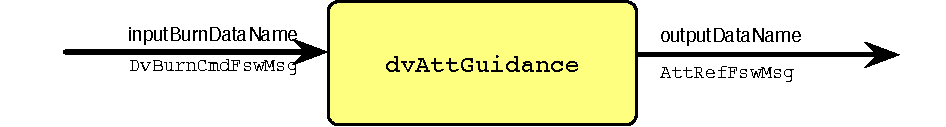
\includegraphics{Figures/moduleImg}
	}
	\caption{Illustration of the module input and output messages.}
	\label{fig:moduleImg}
\end{figure}


\section{Model Description}
\subsection{General Functionality}
The purpose of this module is to create an attitude reference frame suitable for an orbit trajectory correction burn that has a constantly rotating direction.  Assume the initial burn direction is given by $\Delta \bm v$ as illustrated in Figure~\ref{fig:concept}.  The module assumes that the burn direction is always along the current reference frame 1 axis.  If this is not the case, the {\tt attTrackingError} module can be setup to align a different body frame with $\cal R$.  

While the following developments are done in a vectorial manner, all vector components are assumed to be taken with respect to a common inertial frame. 

\begin{figure}[htb]
	\centerline{
	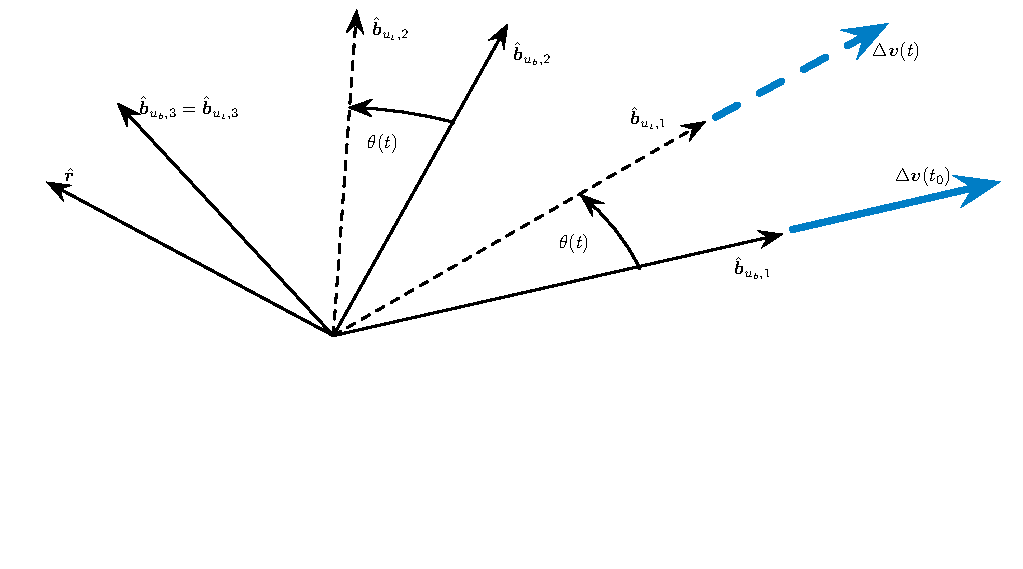
\includegraphics[]{Figures/concept}
	}
	\caption{Burn frame unit vector Illustration.}
	\label{fig:concept}
\end{figure}

\subsection{Base Burn Frame Definition}
The current burn frame is developed in a two-stage process.  First a base frame is developed which is then rotated about the 3rd axis.  Let ${\cal B}_{u,b} = \{\hat{\bm b}_{u_{b},1}, \hat{\bm b}_{u_{b},2}, \hat{\bm b}_{u_{b},3} \}$ be the inertially fixed base burn frame.  The DCM of ${\cal B}_{u,b}$ relative to an inertial frame $\cal N$ is defined as
\begin{equation}
	\label{eq:dvAttGuid0}
	[B_{u,b}N] = \begin{bmatrix}
		\leftexp{N}{\hat{\bm b}_{u_{b},1}}^{T} \\
		\leftexp{N}{\hat{\bm b}_{u_{b},2}}^{T} \\
		\leftexp{N}{\hat{\bm b}_{u_{b},3}}^{T} 		
	\end{bmatrix}
\end{equation}

The first base vector is defined as the normalized $\Delta\bm v$ direction using
\begin{equation}
	\label{eq:dvAttGuid1}
		\hat{\bm b}_{u_{b},1} = \frac{\Delta\bm v}{|\Delta \bm v|}
\end{equation}

To create a full three-dimensional reference frame, a vector $\hat{\bm r}$ is provided in the input message.  The second base Burn frame vector is then defined as
\begin{equation}
	\label{eq:dvAttGuid2}
		\hat{\bm b}_{u_{b},2} = \frac{\hat{\bm r} \times \Delta\bm v}{|\hat{\bm r} \times \Delta \bm v|}
\end{equation}
The final base frame vector is then defined as
\begin{equation}
	\label{eq:dvAttGuid3}
		\hat{\bm b}_{u_{b},3} = \frac{ \hat{\bm b}_{u_{b},1} \times \hat{\bm b}_{u_{b},2}}{|  \hat{\bm b}_{u_{b},1} \times \hat{\bm b}_{u_{b},2} |}
\end{equation}

Note that if $\hat{\bm r}$ and $\Delta\bm v$ are orthogonal to begin with, then $\hat{\bm r} = \hat{\bm b}_{u_{b},3}$.  In this case the $\hat{\bm r}$ vector defines the axis about which the $\Delta \bm v$ vector will rotate.  


\subsection{Burn Time}
The input message contains a time tag $t_{\text{start}}$ when the $\Delta\bm v$ burn is to begin.  The time since this start time is thus evaluated using
\begin{equation}
	\label{eq:dvAttGuid4}
		\Delta t = t - t_{\text{start}}
\end{equation}
where $t$ is the current time. A negative signed $\Delta t$ is a valid burn duration and corresponds to a rotation towards the nominal attitude at the start of the burn.

\subsection{Current Burn Frame}
The current burn frame is defined as ${\cal B}_{u,t} = \{\hat{\bm b}_{u_{t},1}, \hat{\bm b}_{u_{t},2}, \hat{\bm b}_{u_{t},3} \}$.  It differs from the base burn frame through a third base-frame axis rotation.  The rotation rate $\dot\theta$ is given in the input message as {\tt dvRotVecMag}.  The current angle $\theta$ is 
\begin{equation}
	\label{eq:dvAttGuid5}
		\theta(t) = \dot\theta \Delta t
\end{equation}

The DCM going from the base to the current burn frame is 
\begin{equation}
	\label{eq:dvAttGuid6}
	[B_{u,t}B_{u,b}] = \begin{bmatrix}
		\hfill\cos\theta & \sin\theta & 0 \\
		-\sin\theta & \cos\theta & 0 \\
		0 & 0 & 1
	\end{bmatrix}
\end{equation}
The final output reference frame is then computed as
\begin{equation}
	\label{eq:dvAttGuid7}
	[RN] = [B_{u,t}N] =  [B_{u,t}B_{u,b}] [B_{b,t}N] 
\end{equation}
which is mapped into the equivalent $\bm\sigma_{R/N}$ MRP set for the output message. 

The reference frame angular velocity vector is computed as follows.  Note that because ${\cal B}_{u,b}$ is inertially fixed then $\bm\omega_{B_{u,b}/N} = \bm 0$.  The angular velocity vector between the current and the base burn frame is
\begin{equation}
	\label{eq:dvAttGuid8}
	\bm\omega_{B_{u,t}/B_{u,b}} = \dot\theta \hat{\bm b}_{u_{b},3} = \dot\theta \hat{\bm b}_{u_{t},3}
\end{equation}
The desired inertial reference frame vector is then given by 
\begin{equation}
	\label{eq:dvAttGuid9}
	\bm\omega_{R/N} = \bm\omega_{B_{u,t}/N} = \bm\omega_{B_{u,t}/B_{u,b}}+ \bm\omega_{B_{u,b}/N} = \dot\theta \hat{\bm b}_{u_{t},3}
\end{equation}

As $\dot\theta$ is constant and $\hat{\bm b}_{u_{t},3}$ is inertially fixed, the reference angular acceleration is zero.
\begin{equation}
	\label{eq:dvAttGuid10}
	\dot{\bm\omega}_{R/N} = \dot{\bm\omega}_{B_{u,t}/N} = \bm 0
\end{equation}




